\chapter{Ajout des fonctionnalités}


\section{Navigation}
\noindent La navigation est une fonctionnalité très utilisée par les développeurs.
Elle permet de se déplacer dans le code source d'un projet.
Dans le cas d'un projet Prolog, il est important de pouvoir naviguer entre les différents prédicats, leurs usages et leur définitions.
\newdoubleline
Dans le cas d'un language comme Prolog, il est possible de définir plusieurs prédicats avec le même nom mais avec une arité (nombre d'arguments) différente :

\begin{lstlisting}
    predicat(A).
    predicat(A, B).
    predicat(A, B, C).
\end{lstlisting}

La navigation devra donc être consciente de l'arité du prédicat afin de pouvoir naviguer entre les différentes définitions du prédicat mais aussi lors de la recherche de l'utilisation de celui-ci dans le code.
\\ Ceci sera également valable plus tard, lors du refactoring.

\subsection{Goto Declaration}
\noindent Cette partie plus spécifique parlera de la fonctionnalité Goto Declaration.
Cette fonctionnalité permet de naviguer vers la définition d'un prédicat.
Pour cela, il faut sélectionner le prédicat et appuyer sur Ctrl+B (ou Cmd+B sur Mac).
La définition du prédicat s'ouvrira alors dans un nouvel onglet s'il existe.
Si le prédicat est défini à plusieurs endroits, un menu sous forme de popup s'ouvrira et permettra de choisir la définition à ouvrir.
\newdoubleline
\noindent \textbf{Réalisation dans le code}
\\
\noindent La réalisation n'a pas été de tout repos.
En effet, le peu de documentation et d'exemples sur le sujet a rendu la tâche difficile mais finalement réalisable.
\\
\\

\noindent Cheminement:
\begin{enumerate}
    \item Recherche d'exemples sur GitHub et dans la documentation de JetBrains
    \item Création d'une classe \("\)ch.heiafr.intelliprolog.reference.PrologGotoDeclarationHandler\("\)
    \item Méthode de recherche d'inclusion de fichiers
    \item Méthode de recherche des définitions
    \item Méthode qui permet de \("\)matcher\("\) un prédicat avec une définition
\end{enumerate}

\noindent \textbf{Méthode permettant d'extraire le prédicat défini dans la "PrologSentence"}

\begin{lstlisting}[label={lst:method_find_predicate_in_sentence}, caption={Méthode permettant d'extraire le prédicat défini dans la "PrologSentence"}]
public static PsiElement findDefinition(PrologSentence sentence) {

    if (sentence == null) {
        return null;
    }

    //Multiple cases
    Class<?>[][] searchPatterns = new Class[][]{{
            // 1. test :- test2. => atom used as predicate name
            PrologSentence.class, PrologOperation.class, PrologNativeBinaryOperation.class, PrologBasicTerm.class, PrologAtom.class}, {
            // 2. test(A) :- test2. => compound used as predicate name
            PrologSentence.class, PrologOperation.class, PrologNativeBinaryOperation.class, PrologBasicTerm.class, PrologCompound.class}, {
            // 3. test(X). => compound without definition
            PrologSentence.class, PrologCompound.class}, {
            // 4. test. => atom without definition
            PrologSentence.class, PrologAtom.class}};


    for (Class<?>[] searchPattern : searchPatterns) {
        var definition = patternFitPsiElement(sentence, searchPattern);

        if (definition != null) {
            return definition; //Found a definition
        }
    }

    //If not found, return null
    return null;
}
\end{lstlisting}

\noindent Le fonctionnement de cette méthode est le suivant:
\begin{enumerate}
    \item Pour une certaine "PrologSentence" en entrée, on va tester plusieurs cas possibles :
    \begin{enumerate}
        \item test :- test2. => c'est un simple atom qui est défini
        \item test(A) :- test2. => c'est un compound qui est défini
        \item test(X). => c'est un compound qui est défini mais enoncé en tant que fait
        \item test. => c'est un atom qui est défini mais enoncé en tant que fait
    \end{enumerate}
    \item Si le cas est trouvé, on récupère le prédicat correspondant
    \item Sinon, on retourne null
\end{enumerate}
\textbf{Méthode permettant de trouver tous les fichiers inclus récursivement}
\begin{lstlisting}[label={lst:method_find_all_included_files}, caption={Méthode permettant de trouver tous les fichiers inclus récursivement}]
public static Collection<PsiElement> findEveryImportedFile(PsiElement elt, Collection<String> files) {
    if (elt == null) {
        return new ArrayList<>();
    }

    Collection<String> paths = PsiTreeUtil.collectElementsOfType(elt.getContainingFile(), PrologSentence.class).stream()
            .map(ReferenceHelper::findIncludeStatement)// Find the first compound name which is the predicate name
            .filter(Objects::nonNull) //Prevent null values
            .map(ReferenceHelper::extractQuotedString)//Extract the quoted string
            .filter(Objects::nonNull)//Prevent null values
            .filter(s -> !files.contains(s)) //Filter out already visited files
            .collect(Collectors.toList()); //Collect to list

    files.addAll(paths); //Add the new paths to the list of visited files to prevent infinite recursion

    Collection<PsiElement> psiFiles = new ArrayList<>(); //Create a new list of psi files
    for (String path : paths) {
        PsiElement rootElt = pathToPsi(elt, path); //Get the psi element from the path
        psiFiles.add(rootElt); //Add the psi element to the list
        psiFiles.addAll(findEveryImportedFile(rootElt, files)); //Find imported files recursively
    }
    return psiFiles;
}
\end{lstlisting}

\noindent Le fonctionnement de cette méthode est le suivant:
\begin{enumerate}
    \item On recherche toutes les "PrologSentence" du fichier
    \item Pour chaque "PrologSentence", on va chercher le prédicat "include"
    \item Si le prédicat est trouvé, on va chercher le chemin du fichier inclus
    \item Si le chemin n'a pas déjà été visité, on va chercher le fichier correspondant
    \item Si le fichier est trouvé, on va chercher tous les fichiers inclus dans ce fichier de manière récursive
    \item On retourne la liste des fichiers trouvés
\end{enumerate}


\begin{figure}[H]
    \centering
    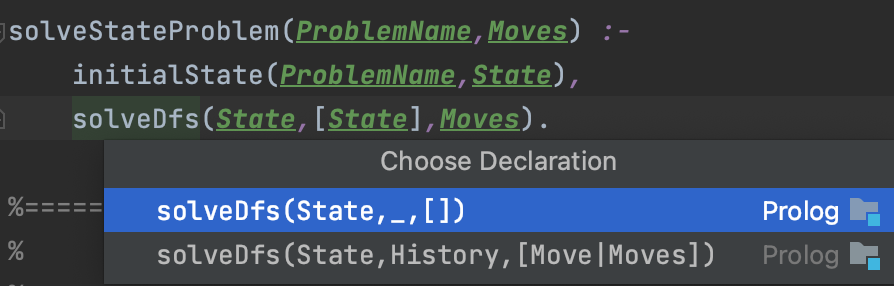
\includegraphics[width=0.8\textwidth]{images/Goto_Declaration.png}
    \caption{Déclaration d'un prédicat}
    \label{fig:definition}
\end{figure}

\subsection{Find usage}
\noindent Pour la recherche d'utilisation, c'est un peu plus simple car certaines méthodes sont déjà implémentées lors de la réalisation du "Goto declaration".
\newdoubleline
En revanche, la recherche doit être exécutée dans un thread séparé pour éviter de bloquer l'IDE pendant la recherche. Si ce n'est pas le cas, une exception est levée automatiquement par l'IDE afin d'interrrompre la méthode.
\newdoubleline
Le fonctionnement est le suivant:
\begin{enumerate}
    \item On récupère le prédicat à rechercher
    \item On lance la recherche dans un thread séparé afin de ne pas bloquer l'IDE
    \item On récupère tous les fichiers .pl
    \item On filtre en fonction de la portée désirée (choisi par l'utilisateur)
    \item On filtre et on retourne les résultats sous forme de UsageInfo
    \item Le Thread s'arrête et les résultats sont affichés
\end{enumerate}

\noindent \textbf{Lancement d'un thread séparé}
\begin{lstlisting}[label={lst:method_find_usages}, caption={Lancement d'un thread séparé}]
public class PrologCustomUsageSearcher extends CustomUsageSearcher {

    @Override
    public void processElementUsages(@NotNull PsiElement element,
                @NotNull Processor<? super Usage> processor, @NotNull FindUsagesOptions options) {

        Application app = ApplicationManager.getApplication(); // get the application

        app.runReadAction(new FindPrologCompoundNameRunnable(element, processor, options));
    }

    private static class FindPrologCompoundNameRunnable implements Runnable {
        private final PsiElement element;
        private final Processor<? super Usage> processor;
        private final FindUsagesOptions options;

        public FindPrologCompoundNameRunnable(PsiElement elt, Processor<? super Usage> processor, FindUsagesOptions options) {
            //Code here
        }

        @Override
        public void run() {
            //Code here
        }
    }
}
\end{lstlisting}

\begin{figure}[H]
    \centering
    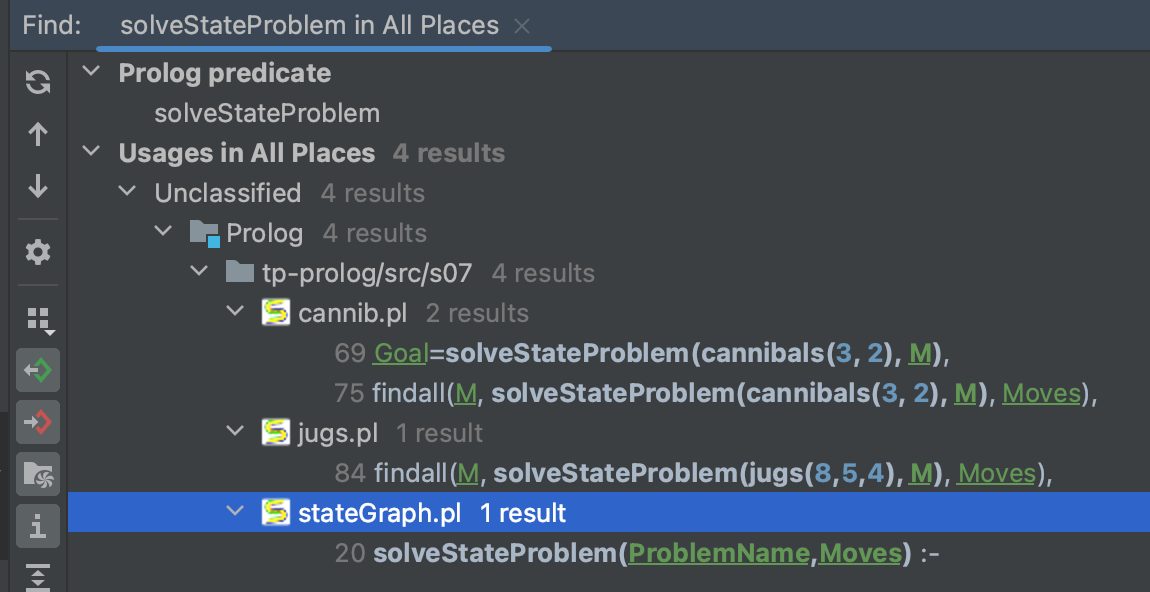
\includegraphics[width=0.8\textwidth]{images/Find_Usage.png}
    \caption{Recherche d'utilisation d'un prédicat}
    \label{fig:usage}
\end{figure}


\section{Refactoring}
\noindent Le refactoring est une fonctionnalité qui permet de modifier le code de manière automatique comme par exemple renommer une variable, une méthode, etc.
C'est une fonctionnalité très appréciée des développeurs car elle permet de gagner du temps et d'éviter les erreurs de frappe ou simplement les oublis lors de la modification du code.
\newdoubleline
Dans notre cas, seul la partie renommage d'un prédicat, d'un atome ou d'une variable nous intéresse.
En effet, il est fréquent de renommer un prédicat ou une variable dans un fichier Prolog et il est important de renommer
toutes les occurrences de ce prédicat ou de cette variable dans tous les fichiers inclus.

\subsection{Renommer un prédicat}
\noindent Pour renommer un prédicat, il faut d'abord récupérer le prédicat à renommer.
Ensuite, il faut récupérer tous les fichiers inclus dans le fichier courant ainsi que tous les fichiers inclus dans ces
fichiers inclus et ainsi de suite.
\newdoubleline
Il faut ensuite remplacer toutes les occurrences du prédicat par le nouveau nom.
\newdoubleline

Exemple d'un renommage de prédicat:

\begin{figure}[H]
    \centering
    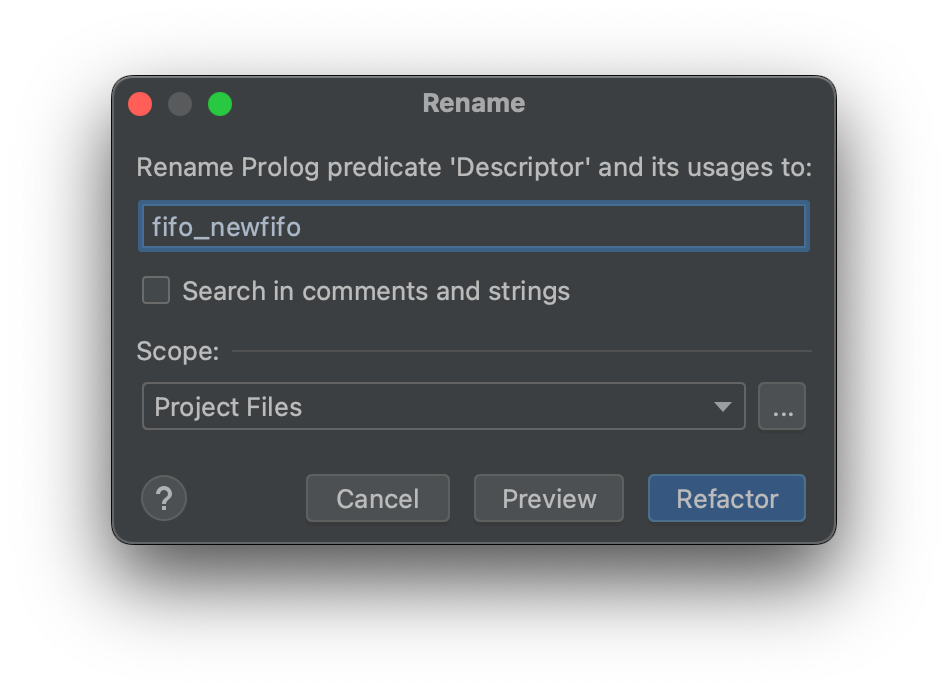
\includegraphics[width=0.8\textwidth]{images/Refactor_window.png}
    \caption{Fenêtre de renommage d'un prédicat}
    \label{fig:refactor_window}
\end{figure}

\begin{figure}[H]
    \centering
    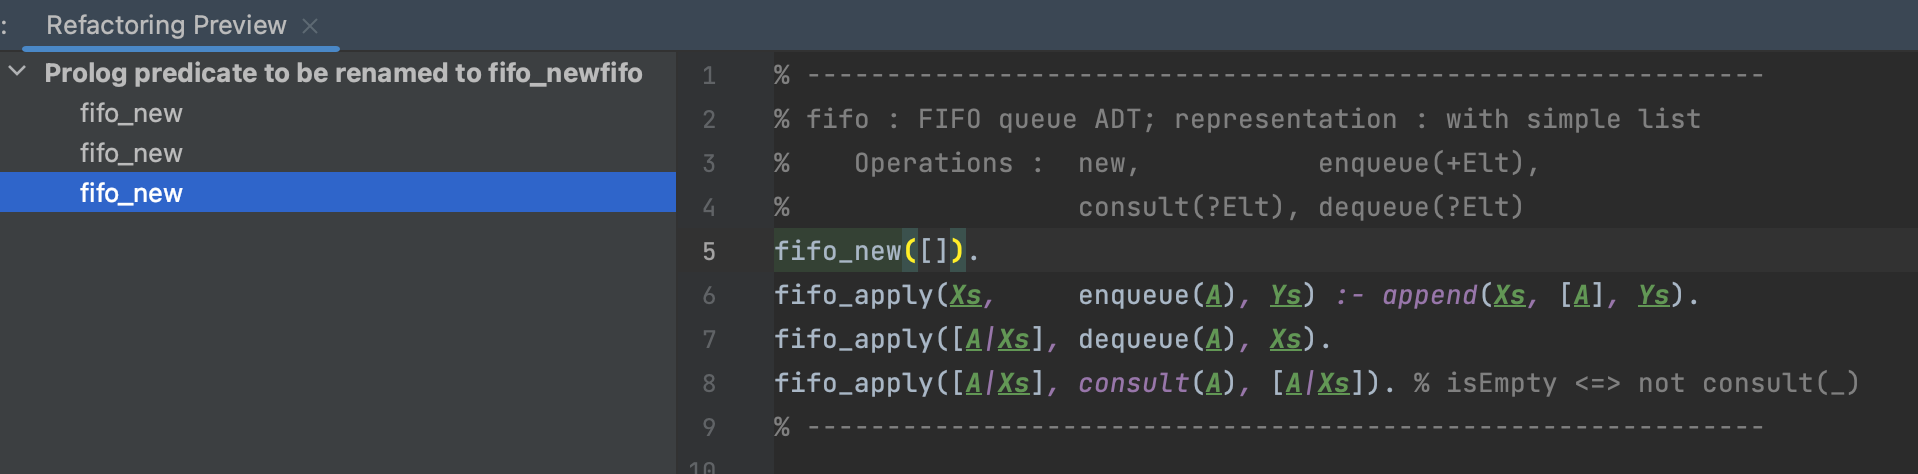
\includegraphics[width=0.8\textwidth]{images/Refactoring_preview.png}
    \caption{Aperçu du refactoring}
    \label{fig:refactor_preview}
\end{figure}

\subsection{Renommer une variable}
\noindent Pour ce qui est du renommage d'une variable, la portée du refactoring est limitée à la phrase Prolog dans laquelle se trouve la variable.
\newdoubleline
Le fonctionnement est similaire à celui du renommage d'un prédicat, à la différence que l'on ne va pas chercher en dehors de la phrase Prolog dans laquelle se trouve la variable.

\subsection{Fonctionnement du renommage}
\noindent Le fonctionnement du renommage est le suivant:
\begin{enumerate}
    \item On récupère le prédicat ou la variable à renommer
    \item On récupère tous les fichiers inclus dans le fichier courant
    \item On récupère tous les fichiers inclus dans ces fichiers inclus et ainsi de suite
    \item On affiche un aperçu des modifications
    \item On remplace toutes les occurrences du prédicat ou de la variable par le nouveau nom
\end{enumerate}

\noindent La classe qui gère le renommage est la suivante \textbf{PrologRenamePsiElementProcessor}.
Voici une brève description des méthodes de cette classe héritée de \textbf{RenamePsiElementProcessor}:
\begin{enumerate}
    \item \textbf{canProcessElement}: Cette méthode permet de vérifier si l'élément peut être renommé. Dans notre cas, on vérifie si l'élément est un prédicat ou une variable.
    \item \textbf{prepareRenaming}: Cette méthode permet de préparer le renommage. Dans notre cas, on récupère tous les prédicats de tous les fichiers touchés par le renommage.
    \item \textbf{renameElement}: Cette méthode permet de renommer chaque prédicat/variable.
\end{enumerate}


\section{Affichage des erreurs et warnings}
\noindent Lors de la compilation d'un fichier Prolog, il est possible que des erreurs ou des warnings apparaissent
qui ne sont pas détectés plus tôt car ce ne sont pas des erreurs de syntaxe.
\newdoubleline
Par exemple, il est possible d'avoir une erreur de prédicats non définis ou une erreur de variables non définies ou simplement des avertissements par rapport à des variables "Singletons".

\subsection{L'idée}
\noindent L'idée est de récupérer les erreurs et les warnings de la compilation du fichier Prolog et de les afficher dans l'éditeur Prolog.
\newdoubleline
Ceci implique différentes contraintes:
\begin{enumerate}
    \item Il faut prendre en compte que la compilation doit avoir lieu en temps réel et en arrière plan.
    \item La compilation doit avoir lieu sur macOS, Linux et Windows.
    Ce qui implique de mettre en place un système multi-plateforme.
    \item La compilation doit aussi être dans un thread séparé pour ne pas bloquer l'interface et ne pas ralentir l'éditeur.
\end{enumerate}

\subsection{La mise en pratique}
\noindent Pour la compilation, nous utiliserons le SDK relatif au projet ouvert.
\newdoubleline
Pour l'aspect compilation en temps réel, JetBrains propose une classe nommée "ExternalAnnotator" qui permet de faire des annotations externes.
\newdoubleline
Cette classe permet de faire des annotations externes, notamment à l'aide d'un thread séparé. La classe se présente comme suit:
\begin{enumerate}
    \item \textbf{collectInformation}: Cette méthode permet de récupérer les informations afin de générer les annotations.
    C'est dans cette partie que le lancement de la compilation aura lieu.
    \item \textbf{doAnnotate}: Cette méthode permet de générer les annotations pour chaque ligne.
\end{enumerate}

\noindent Voici le code permettant de récupérer un processus de compilation Prolog:
\begin{lstlisting}[label={lst:get_prolog_process}, caption={Méthode de créer un processus de compilation Prolog}, language=java]
    public static Process getProcess(Path compiler, Path filePath) throws IOException, CantRunException {
        Process p;
        BufferedWriter writer;

        if (SystemInfo.isWindows) {
            p = Runtime.getRuntime().exec("cmd.exe /min");
            writer = new BufferedWriter(new java.io.OutputStreamWriter(p.getOutputStream()));
            writer.write("set LINEDIT=gui=no"); //Prevent windows from opening a console
            writer.newLine();
            writer.write(compiler.toString()); //Launch the compiler
            writer.newLine();
            writer.flush(); //Flush the stream
        } else {
            p = Runtime.getRuntime().exec(compiler.toString());
            writer = new BufferedWriter(new java.io.OutputStreamWriter(p.getOutputStream()));
        }

        writer = new BufferedWriter(new java.io.OutputStreamWriter(p.getOutputStream()));
        String normalizedFilePath = filePath.toString().replace("\\", "/"); //Mandatory for windows
        String goal = "consult('" + normalizedFilePath + "').";
        writer.write(goal);
        writer.newLine();
        writer.flush();
        writer.close();
        return p;
    }
\end{lstlisting}

\noindent Au final, voici le résultat en action dans l'éditeur :
\begin{figure}[h]
    \centering
    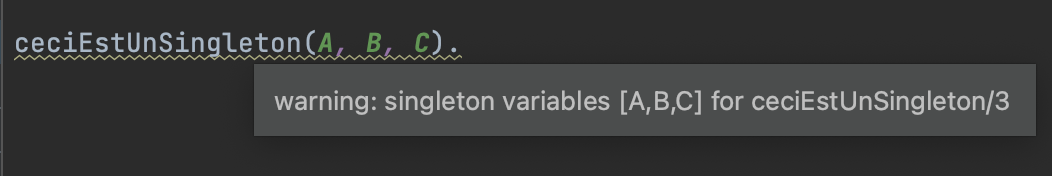
\includegraphics[width=0.8\textwidth]{images/background_compilation.png}
    \caption{Affichage d'avertissement grâce à la compilation}
    \label{fig:compilation_warnings}
\end{figure}

\section{Auto-complétion}


\section{Formatage du code}


\section{Déploiement du plugin}
